\section{Functionaliteit}

\textit{In dit hoofdstuk wordt er onderzocht welke functionaliteiten de netwerken ondersteunen die uitgelicht zijn in het vorige hoofdstuk. Er wordt gekeken welke gevaren er kunnen optreden in het netwerk aan de hand van het opstellen van een threat model.}

\paragraph{Architectuur}
Bitcoin is een netwerk waarin geen coördinerende rollen zijn. Elke deelnemer van het netwerk heeft een complete replica van alle informatie die benodigd is voor het verifiëren van de validiteit van binnenkomende transacties. Er zijn verschillende services die het netwerk faciliteert die kort toegelicht zijn in \ref{blockchain_node_types}, twee daarvan zijn met name belangrijk voor de beschrijving van het netwerk: netwerk routing, en het mining proces. In de basis van het netwerk staan de transacties die op abstract niveau bitcoins van een of meer accounts naar een of meer bestemmingsaccounts overmaken. Een \gls{account}, in de context van het bitcoin netwerk, is een combinatie van een public- en private key, waarbij de public key als identificatie van de \gls{account} gebruikt wordt. Om een transactie te versturen wordt de transactie gesigneerd met de private key van de \gls{account} die de transactie wilt uitvoeren. 
\begin{wrapfigure}{r}{0.6\textwidth}
  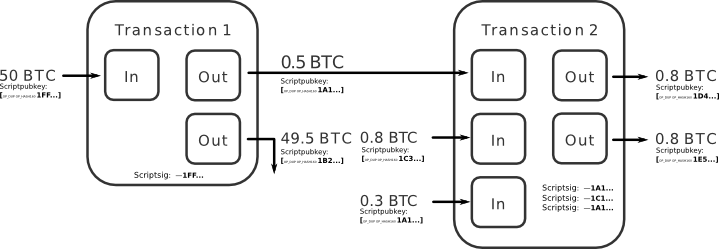
\includegraphics[width=0.6\textwidth]{utxo}
  \caption[UTXO-model]{Voorbeeld van het UTXO-model zoals in gebruik bij Bitcoin, bron: http://news.8btc.com/thoughts-on-bytom-design-extension-of-utxo-structure.}
  \label{utxo_model}
\end{wrapfigure}

Transacties bestaan uit een input en output. In plaats van het aggregeren van een balans voor elk \gls{account}, wordt er bijgehouden wat de output van een transactie is. De balans is hierbij de som van alle openstaande outputs van het desbetreffend \gls{account}. In fig. \ref{utxo_model} is te zien hoe dit in zijn werk gaat. Een onderdeel van de services die de \glspl{node} binnen het netwerk aanbieden is het valideren van transacties. Hierbij worden drie onderdelen gevalideerd:

\begin{itemize}

  \item Een output mag maar één keer geclaimd zijn.
  \item Nieuwe outputs worden alleen gecreëerd door een transactie.
  \item De som van alle waardes van de geclaimde outputs moet groter zijn als de totale som van de nieuwe gecreëerde outputs.
\end{itemize}

Wanneer dit het geval is wordt de transactie geaccepteerd en opgenomen in de lokale replica van de blockchain. Over tijd kan het voorkomen dat de replica van verschillende \glspl{node} inconsistent worden, waarbij het kan voorkomen dat er twee of meer transacties dezelfde coin meerdere malen uitgeeft. Dit staat bekend als \gls{double_spending} \citep{6688704}.

\clearpage
Een nieuw block wordt gecreëerd door het uitvoeren van het mining proces. Dit wordt uitgevoerd door zogenaamde \glspl{miner} node. Om te bepalen welke \gls{node} verantwoordelijk is voor het volgende block moet er een oplossing gevonden worden voor het proof-of-work. Dit proces zorgt ervoor dat er een beslissing gemaakt wordt over de volgorde van de transacties, en dat de inhoudt van een block niet aangepast kan worden omdat dit in directe verbinding staat met het gedane \acrshort{PoW}.

\paragraph{Discovery protocol}

Om het het netwerk te betreden worden er DNS servers benaderd waarbij gebruik wordt gemaakt van het TCP protocol. Deze DNS servers worden in stand gehouden door vrijwilligers en geven een willekeurige set aan \glspl{bootstrap_node} terug die actief zijn in het netwerk. Wanneer de \gls{node} toegetreden is tot het netwerk wordt er een \gls{peer_list} bijgehouden met alle \glspl{node} waarmee er connectie is gelegd. Deze \gls{peer_list} wordt gebruikt om connectie te leggen bij een eerstvolgende toetreding tot het netwerk.

\paragraph{Informatie propagatie}

Voor het updaten en synchroniseren van de blockchain worden er \acrfull{tx} en block berichten verstuurd. Om tegen te gaan dat \acrshort{tx}- en block berichten verstuurd worden naar \glspl{node} die al afweten van deze informatie, wordt er een \textit{inv} bericht verstuurd wanneer een transactie of een block volledig geverifieerd is. Het \textit{inv} bericht bevat een lijst van transactie- en block hashes die reeds ontvangen zijn door de verstuurder en die beschikbaar zijn om opgehaald te worden. 
\begin{wrapfigure}{r}{0.5\textwidth}
  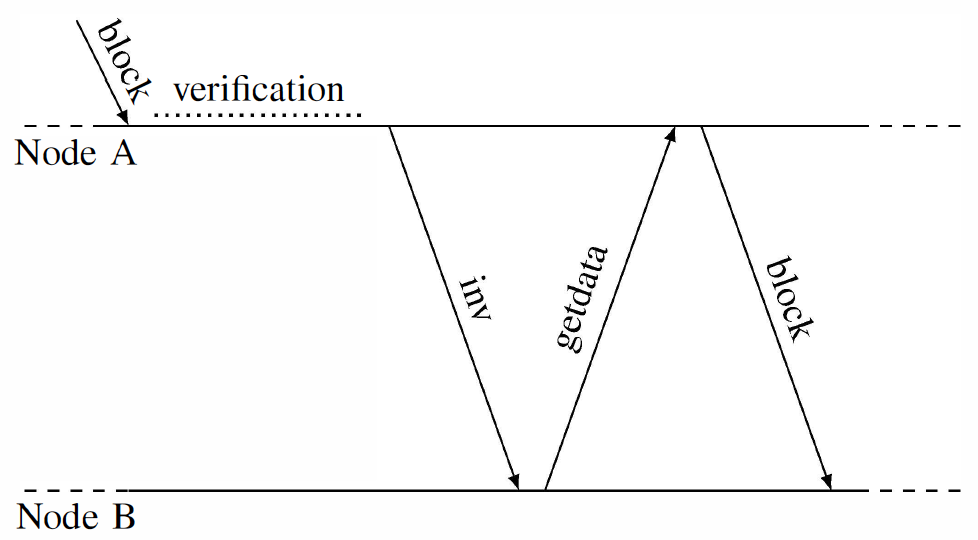
\includegraphics[width=0.5\textwidth]{bitcoin_information_propagation_0}
  \caption[Communicatie tussen deelnemers in Bitcoin]{Berichten die verzonden worden om informatie over een block uit te wisselen \citep[p.~4]{6688704}.}
  \label{bitcoin_information_propagation_0}
\end{wrapfigure}

Wanneer een \gls{node} deze informatie wilt ontvangen (bijv. omdat het de informatie nog niet heeft), wordt er een \textit{getdata} bericht verstuurd naar de verstuurder van het \textit{inv} bericht, met daarin de hashes van de informatie die de \gls{node} wilt hebben. Fig. \ref{bitcoin_information_propagation_0} visualiseert dit proces.
\clearpage
\paragraph{Architectuur}
Net zoals bij Bitcoin zijn de transacties de kern van de implementatie, waarbij er wederom gebruik wordt gemaakt van het \gls{UTXO} zoals beschreven bij de architectuur van Bitcoin. 
De architectuur van het Cardano netwerk bestaat uit drie soorten \glspl{node} die fundamenteel zijn voor de werking van het protocol: \textit{core}, \textit{relay} en \textit{edge} \glspl{node}.\textit{Core \glspl{node}} zijn de kern van het netwerk. Het zijn de enige \glspl{node} die geselecteerd kunnen worden om \gls{slot_leader} te worden, waardoor het de enige \glspl{node} zijn die een block kunnen creëren.
\textit{Relay \glspl{node}} worden gezien als de proxy tussen core \glspl{node} en het internet. Ze hebben geen stake in het netwerk, waardoor ze makkelijk te verplaatsten of veranderd kunnen worden.
\textit{Edge \glspl{node}} zijn de simpele \glspl{node} die iedereen kan uitvoeren. Deze \glspl{node} kunnen transacties aanmaken binnen het netwerk en aanbieden aan \textit{core} \glspl{node} via de \textit{relay} \glspl{node} \citep[Topology]{cardano_wiki}.

\paragraph{Discovery protocol}
\begin{wrapfigure}{r}{0.6\textwidth}
  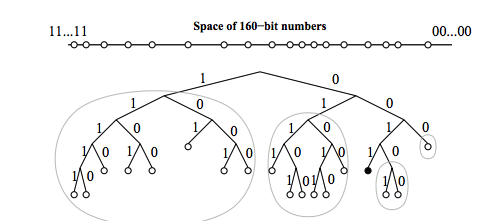
\includegraphics[width=0.6\textwidth]{kademlia}
  \caption[Kademlia Binary Tree]{Binary Tree zoals in gebruik bij het Kademlia protocol, \cite{maymounkov2002kademlia}.}
  \label{kademlia_binary_tree}
\end{wrapfigure}

Om het netwerk te betreden wordt er gebruik gemaakt van een bestaand protocol genaamd Kademlia, wat gebaseerd is op het gebruik van een \acrfull{DHT} architectuur. Elke node wordt behandeld als een tak in een Binary Tree waarbij de positie van een \gls{node} bepaald wordt door een unieke prefix van de identificatie code van een \gls{node}. In fig. \ref{kademlia_binary_tree} is de positie van een \gls{node} met de prefix 0011 te zien. Het protocol garandeert dat elke \gls{node} in verbinding staat met een andere \gls{node}. Met deze garantie kan elke \gls{node} een andere \gls{node} lokaliseren aan de hand van de identificatie code \citep[p.~2]{maymounkov2002kademlia}.

\subsubsection{Informatie propagatie}
Berichten worden verstuurd voor het uitwisselen van informatie tussen deelnemers. Hierbij zijn drie abstracte types gedefinieerd: \textit{inv}, \textit{req} en \textit{data}. Net zoals bij Bitcoin wordt de \textit{inv} message gebruikt om aan te geven dat er data beschikbaar is. Het \textit{req} bericht wordt vervolgens gebruikt om beschikbare data op te vragen. De data wordt vervolgens verstuurd via een \textit{data} message. Berichten die bijvoorbeeld een block versturen zijn nader gespecificeerde \textit{data} berichten. Op deze drie types zijn alle berichten in het netwerk gebaseerd, bijvoorbeeld is het \textit{MsgBlock} bericht, die block informatie uitwisselt, gebaseerd op een \textit{data} bericht \citep{cardano_wiki:csl_app_level}. Een bericht kan verstuurd worden naar drie verschillende mediums: het versturen van een bericht naar een \gls{node}, de buren, en het gehele netwerk. Naar welk medium het bericht wordt verstuurd is opgenomen in de header van een bericht.

\clearpage
https://steemit.com/eos/@trogdor/eos-vs-ethereum-for-dummies

De blockchain implementatie EOS werkt toe naar een operating systeem speciaal voor blockchain toepassingen. In eerste instantie zal er een Blockchain gerealiseerd worden die dient als proof-of-concept van het ontwerp. In dit proof-of-concept is er een eerste versie gerealiseerd die het mogelijk maakt voor developers om een eigen applicatie op het EOS netwerk te creëren. Hierbij is de focus gelegd het faciliteren van functionaliteiten die betrekking hebben op account permissies, authenticatie en de communicatie tussen het internet en het netwerk. Er wordt gespeculeerd dat EOS een sterke concurrent van Ethereum zal worden als het gaat om Blockchain als een developer platform.

\paragraph{Architectuur}

EOS maakt gebruik van aanpak waarbij extensies op de basis componenten (e.g. het netwerk, de 'chain', etc.) gerealiseerd worden als plugins. Dit maakt het zodat het protocol makkelijk te wijzigen is in de toekomst. 
\paragraph{Discovery protocol}

\subsubsection{Informatie propagatie}
\clearpage
\paragraph{Architectuur}

Monero maakt gebruik van \acrfull{I2P} protocol. Het \acrshort{I2P} protocol stelt het netwerk in staat om deelnemers te beschermen tegen een zekere mate van verkeer; waarbij de identiteit van de verstuurder en ontvanger verborgen wordt, terwijl er gebruik gemaakt wordt van encryptiestandaarden om de inhoud van berichten te verbergen en te garanderen dat het bericht aankomt \citep{zantout2011i2p}. Het protocol ondersteund zowel TCP/IP als UDP/IP communicatie, waarbij de Transport laag in het network van Monero gelimiteerd is aan de mogelijkheden die \acrshort{I2P} ondersteund \citep{moneropedia:kovri}.
De transport laag faciliteert de connectie tussen de verschillende deelnemers in het netwerk. Om vervolgens te kunnen communiceren wordt er gebruik gemaakt van een \gls{tunnel}. Elke deelnemer in het netwerk heeft minimaal twee \Glspl{tunnel}, een voor uitgaand- en inkomend verkeer. Wanneer er communicatie plaatsvind tussen twee deelnemers zullen er vier \glspl{tunnel} aangemaakt worden; twee voor uitgaand verkeerd en twee voor inkomend verkeer \citep{moneropedia:tunnel}. Ook Monero maakt gebruik van het \gls{UTXO}, waarbij er bij iedere transactie twee keys aanwezig zijn; een spend key en een view key. Beide keys zijn onderdeel van een account, waarbij de spend key gebruikt wordt om geld uit te geven, en de view key gebruikt wordt om permissie te geven om de transacties in te zien van een deelnemer. De keys spelen een belangrijke rol in de privacy van de deelnemer omtrent transacties \citep{moneropedia:account}. 

\paragraph{Discovery protocol}

Het discovery protocol in gebruik bij Monero is soortgelijk aan de manier waarop Bitcoin het discovery proces uitvoert. Om het netwerk te bootstrappen wordt er gebruik gemaakt van \glspl{node} die vastgelegd zijn in de broncode, waarna er een lijst van \glspl{peer} wordt teruggegeven aan de deelnemer en de centrale node vergeten wordt. Het is ook mogelijk om zelf deelnemers vast te leggen waarna geprobeerd wordt om connectie te maken.

\paragraph{Informatie propagatie}

Alles binnen het \acrshort{I2P} netwerk wordt gecommuniceerd via berichten. In het onderdeel architectuur is er kort gesproken over \Gls{tunnel} en de functionaliteiten die ermee gerealiseerd wordt. Er zijn twee soorten berichten die verzonden worden: \Gls{tunnel} berichten en \acrfull{I2NP} berichten\footnote{Zie \href{https://geti2p.net/en/docs/protocol/i2np}{"I2NP Specifiation - I2P | Overview"} voor de verschillende types.}. Het proces, zoals beschreven in \cite{moneropedia:message}:

\begin{itemize}
  \setlength\itemsep{-0.7em}
  \item De \Gls{tunnel} verzameld \acrshort{I2NP} berichten en verwerkt ze naar \Gls{tunnel} berichten. Hierbij kan het voorkomen dat \acrshort{I2NP} berichten gefragmenteerd worden omdat ze van variabele grootte zijn, terwijl \Gls{tunnel} berichten een vaste grootte hebben.
  \item De \Gls{tunnel} encrypt de verwerkte data en stuurt het door in de vorm van \Gls{tunnel} berichten.
  \item De deelnemer, en andere deelnemers die deel uitmaken van de \Gls{tunnel}, pakken een laag van de encryptie uit en verifiëren dat het bericht geen duplicaat is en sturen het vervolgens door naar een volgende deelnemer.
  \item Met de tijd zullen de \Gls{tunnel} berichten het eindpunt bereiken waarna ze terug worden gezet naar de originele \acrshort{I2NP} berichten.
\end{itemize}

\clearpage
\section{Gevaren}



\clearpage

% \begin{centering}
%   \begin{table}
%     \makebox[\textwidth]{%
%       \begin{tabular}{@{}l|cccccc@{}}
%         \toprule
%         \textbf{Implementatie} & \textit{Eclipse Attack} & \textit{Majority Attack} & \textit{Sybil Attack} & \textit{Denial of Service} & \textit{Double Spending} & \textit{Nothing at Stake} \\ 
%         \midrule
%         \textit{Bitcoin} & \Rmnum{3} & \Rmnum{3} & \Rmnum{2} & \Rmnum{1} & \Rmnum{2} & ... \\
%         \textit{Cardano} & \Rmnum{5} & \Rmnum{3} & \Rmnum{3} & \Rmnum{2} & \Rmnum{4} & ... \\
%         \textit{EOS} & - &  &  &  &  &  \\
%         \textit{Monero} &  &  &  & ... &  & ... \\
%         \bottomrule
%         \multicolumn{6}{l}{} \Rmnum{1} meerdere keren uitgevoerd, \Rmnum{2} uitgevoerd, \Rmnum{3} theoretisch mogelijk, \Rmnum{4} onbekend, \Rmnum{5} niet mogelijk & \\
%       \end{tabular}
%     }
%     \caption{Indicatie van gevaren in Blockchain implementaties.}
%     \label{my-label}
%   \end{table}
% \end{centering}

\paragraph{Architectuur}
Bitcoin is een netwerk waarin geen coördinerende rollen zijn. Elke deelnemer van het netwerk heeft een complete replica van alle informatie die benodigd is voor het verifiëren van de validiteit van binnenkomende transacties. Er zijn verschillende services die het netwerk faciliteert die kort toegelicht zijn in \ref{blockchain_node_types}, twee daarvan zijn met name belangrijk voor de beschrijving van het netwerk: netwerk routing, en het mining proces. In de basis van het netwerk staan de transacties die op abstract niveau bitcoins van een of meer accounts naar een of meer bestemmingsaccounts overmaken. Een \gls{account}, in de context van het bitcoin netwerk, is een combinatie van een public- en private key, waarbij de public key als identificatie van de \gls{account} gebruikt wordt. Om een transactie te versturen wordt de transactie gesigneerd met de private key van de \gls{account} die de transactie wilt uitvoeren. 
\begin{wrapfigure}{r}{0.6\textwidth}
  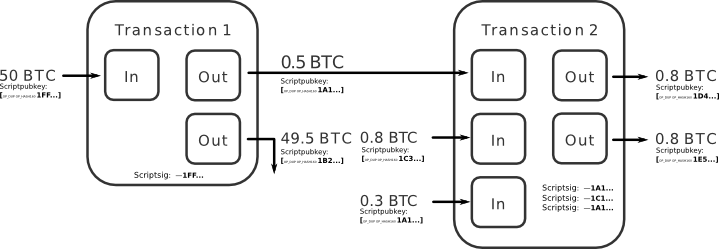
\includegraphics[width=0.6\textwidth]{utxo}
  \caption[UTXO-model]{Voorbeeld van het UTXO-model zoals in gebruik bij Bitcoin, bron: http://news.8btc.com/thoughts-on-bytom-design-extension-of-utxo-structure.}
  \label{utxo_model}
\end{wrapfigure}

Transacties bestaan uit een input en output. In plaats van het aggregeren van een balans voor elk \gls{account}, wordt er bijgehouden wat de output van een transactie is. De balans is hierbij de som van alle openstaande outputs van het desbetreffend \gls{account}. In fig. \ref{utxo_model} is te zien hoe dit in zijn werk gaat. Een onderdeel van de services die de \glspl{node} binnen het netwerk aanbieden is het valideren van transacties. Hierbij worden drie onderdelen gevalideerd:

\begin{itemize}

  \item Een output mag maar één keer geclaimd zijn.
  \item Nieuwe outputs worden alleen gecreëerd door een transactie.
  \item De som van alle waardes van de geclaimde outputs moet groter zijn als de totale som van de nieuwe gecreëerde outputs.
\end{itemize}

Wanneer dit het geval is wordt de transactie geaccepteerd en opgenomen in de lokale replica van de blockchain. Over tijd kan het voorkomen dat de replica van verschillende \glspl{node} inconsistent worden, waarbij het kan voorkomen dat er twee of meer transacties dezelfde coin meerdere malen uitgeeft. Dit staat bekend als \gls{double_spending} \citep{6688704}.

\clearpage
Een nieuw block wordt gecreëerd door het uitvoeren van het mining proces. Dit wordt uitgevoerd door zogenaamde \glspl{miner} node. Om te bepalen welke \gls{node} verantwoordelijk is voor het volgende block moet er een oplossing gevonden worden voor het proof-of-work. Dit proces zorgt ervoor dat er een beslissing gemaakt wordt over de volgorde van de transacties, en dat de inhoudt van een block niet aangepast kan worden omdat dit in directe verbinding staat met het gedane \acrshort{PoW}.

\paragraph{Discovery protocol}

Om het het netwerk te betreden worden er DNS servers benaderd waarbij gebruik wordt gemaakt van het TCP protocol. Deze DNS servers worden in stand gehouden door vrijwilligers en geven een willekeurige set aan \glspl{bootstrap_node} terug die actief zijn in het netwerk. Wanneer de \gls{node} toegetreden is tot het netwerk wordt er een \gls{peer_list} bijgehouden met alle \glspl{node} waarmee er connectie is gelegd. Deze \gls{peer_list} wordt gebruikt om connectie te leggen bij een eerstvolgende toetreding tot het netwerk.

\paragraph{Informatie propagatie}

Voor het updaten en synchroniseren van de blockchain worden er \acrfull{tx} en block berichten verstuurd. Om tegen te gaan dat \acrshort{tx}- en block berichten verstuurd worden naar \glspl{node} die al afweten van deze informatie, wordt er een \textit{inv} bericht verstuurd wanneer een transactie of een block volledig geverifieerd is. Het \textit{inv} bericht bevat een lijst van transactie- en block hashes die reeds ontvangen zijn door de verstuurder en die beschikbaar zijn om opgehaald te worden. 
\begin{wrapfigure}{r}{0.5\textwidth}
  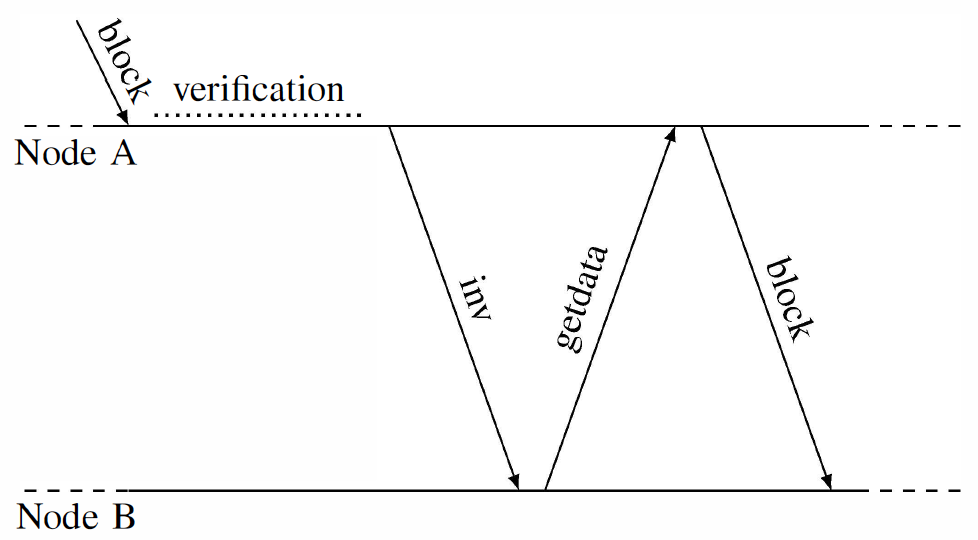
\includegraphics[width=0.5\textwidth]{bitcoin_information_propagation_0}
  \caption[Communicatie tussen deelnemers in Bitcoin]{Berichten die verzonden worden om informatie over een block uit te wisselen \citep[p.~4]{6688704}.}
  \label{bitcoin_information_propagation_0}
\end{wrapfigure}

Wanneer een \gls{node} deze informatie wilt ontvangen (bijv. omdat het de informatie nog niet heeft), wordt er een \textit{getdata} bericht verstuurd naar de verstuurder van het \textit{inv} bericht, met daarin de hashes van de informatie die de \gls{node} wilt hebben. Fig. \ref{bitcoin_information_propagation_0} visualiseert dit proces.
\newpage

\paragraph{Architectuur}
Net zoals bij Bitcoin zijn de transacties de kern van de implementatie, waarbij er wederom gebruik wordt gemaakt van het \gls{UTXO} zoals beschreven bij de architectuur van Bitcoin. 
De architectuur van het Cardano netwerk bestaat uit drie soorten \glspl{node} die fundamenteel zijn voor de werking van het protocol: \textit{core}, \textit{relay} en \textit{edge} \glspl{node}.\textit{Core \glspl{node}} zijn de kern van het netwerk. Het zijn de enige \glspl{node} die geselecteerd kunnen worden om \gls{slot_leader} te worden, waardoor het de enige \glspl{node} zijn die een block kunnen creëren.
\textit{Relay \glspl{node}} worden gezien als de proxy tussen core \glspl{node} en het internet. Ze hebben geen stake in het netwerk, waardoor ze makkelijk te verplaatsten of veranderd kunnen worden.
\textit{Edge \glspl{node}} zijn de simpele \glspl{node} die iedereen kan uitvoeren. Deze \glspl{node} kunnen transacties aanmaken binnen het netwerk en aanbieden aan \textit{core} \glspl{node} via de \textit{relay} \glspl{node} \citep[Topology]{cardano_wiki}.

\paragraph{Discovery protocol}
\begin{wrapfigure}{r}{0.6\textwidth}
  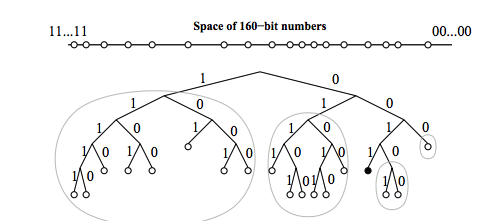
\includegraphics[width=0.6\textwidth]{kademlia}
  \caption[Kademlia Binary Tree]{Binary Tree zoals in gebruik bij het Kademlia protocol, \cite{maymounkov2002kademlia}.}
  \label{kademlia_binary_tree}
\end{wrapfigure}

Om het netwerk te betreden wordt er gebruik gemaakt van een bestaand protocol genaamd Kademlia, wat gebaseerd is op het gebruik van een \acrfull{DHT} architectuur. Elke node wordt behandeld als een tak in een Binary Tree waarbij de positie van een \gls{node} bepaald wordt door een unieke prefix van de identificatie code van een \gls{node}. In fig. \ref{kademlia_binary_tree} is de positie van een \gls{node} met de prefix 0011 te zien. Het protocol garandeert dat elke \gls{node} in verbinding staat met een andere \gls{node}. Met deze garantie kan elke \gls{node} een andere \gls{node} lokaliseren aan de hand van de identificatie code \citep[p.~2]{maymounkov2002kademlia}.

\subsubsection{Informatie propagatie}
Berichten worden verstuurd voor het uitwisselen van informatie tussen deelnemers. Hierbij zijn drie abstracte types gedefinieerd: \textit{inv}, \textit{req} en \textit{data}. Net zoals bij Bitcoin wordt de \textit{inv} message gebruikt om aan te geven dat er data beschikbaar is. Het \textit{req} bericht wordt vervolgens gebruikt om beschikbare data op te vragen. De data wordt vervolgens verstuurd via een \textit{data} message. Berichten die bijvoorbeeld een block versturen zijn nader gespecificeerde \textit{data} berichten. Op deze drie types zijn alle berichten in het netwerk gebaseerd, bijvoorbeeld is het \textit{MsgBlock} bericht, die block informatie uitwisselt, gebaseerd op een \textit{data} bericht \citep{cardano_wiki:csl_app_level}. Een bericht kan verstuurd worden naar drie verschillende mediums: het versturen van een bericht naar een \gls{node}, de buren, en het gehele netwerk. Naar welk medium het bericht wordt verstuurd is opgenomen in de header van een bericht.

\newpage

https://steemit.com/eos/@trogdor/eos-vs-ethereum-for-dummies

De blockchain implementatie EOS werkt toe naar een operating systeem speciaal voor blockchain toepassingen. In eerste instantie zal er een Blockchain gerealiseerd worden die dient als proof-of-concept van het ontwerp. In dit proof-of-concept is er een eerste versie gerealiseerd die het mogelijk maakt voor developers om een eigen applicatie op het EOS netwerk te creëren. Hierbij is de focus gelegd het faciliteren van functionaliteiten die betrekking hebben op account permissies, authenticatie en de communicatie tussen het internet en het netwerk. Er wordt gespeculeerd dat EOS een sterke concurrent van Ethereum zal worden als het gaat om Blockchain als een developer platform.

\paragraph{Architectuur}

EOS maakt gebruik van aanpak waarbij extensies op de basis componenten (e.g. het netwerk, de 'chain', etc.) gerealiseerd worden als plugins. Dit maakt het zodat het protocol makkelijk te wijzigen is in de toekomst. 
\paragraph{Discovery protocol}

\subsubsection{Informatie propagatie}
\newpage

\paragraph{Architectuur}

Monero maakt gebruik van \acrfull{I2P} protocol. Het \acrshort{I2P} protocol stelt het netwerk in staat om deelnemers te beschermen tegen een zekere mate van verkeer; waarbij de identiteit van de verstuurder en ontvanger verborgen wordt, terwijl er gebruik gemaakt wordt van encryptiestandaarden om de inhoud van berichten te verbergen en te garanderen dat het bericht aankomt \citep{zantout2011i2p}. Het protocol ondersteund zowel TCP/IP als UDP/IP communicatie, waarbij de Transport laag in het network van Monero gelimiteerd is aan de mogelijkheden die \acrshort{I2P} ondersteund \citep{moneropedia:kovri}.
De transport laag faciliteert de connectie tussen de verschillende deelnemers in het netwerk. Om vervolgens te kunnen communiceren wordt er gebruik gemaakt van een \gls{tunnel}. Elke deelnemer in het netwerk heeft minimaal twee \Glspl{tunnel}, een voor uitgaand- en inkomend verkeer. Wanneer er communicatie plaatsvind tussen twee deelnemers zullen er vier \glspl{tunnel} aangemaakt worden; twee voor uitgaand verkeerd en twee voor inkomend verkeer \citep{moneropedia:tunnel}. Ook Monero maakt gebruik van het \gls{UTXO}, waarbij er bij iedere transactie twee keys aanwezig zijn; een spend key en een view key. Beide keys zijn onderdeel van een account, waarbij de spend key gebruikt wordt om geld uit te geven, en de view key gebruikt wordt om permissie te geven om de transacties in te zien van een deelnemer. De keys spelen een belangrijke rol in de privacy van de deelnemer omtrent transacties \citep{moneropedia:account}. 

\paragraph{Discovery protocol}

Het discovery protocol in gebruik bij Monero is soortgelijk aan de manier waarop Bitcoin het discovery proces uitvoert. Om het netwerk te bootstrappen wordt er gebruik gemaakt van \glspl{node} die vastgelegd zijn in de broncode, waarna er een lijst van \glspl{peer} wordt teruggegeven aan de deelnemer en de centrale node vergeten wordt. Het is ook mogelijk om zelf deelnemers vast te leggen waarna geprobeerd wordt om connectie te maken.

\paragraph{Informatie propagatie}

Alles binnen het \acrshort{I2P} netwerk wordt gecommuniceerd via berichten. In het onderdeel architectuur is er kort gesproken over \Gls{tunnel} en de functionaliteiten die ermee gerealiseerd wordt. Er zijn twee soorten berichten die verzonden worden: \Gls{tunnel} berichten en \acrfull{I2NP} berichten\footnote{Zie \href{https://geti2p.net/en/docs/protocol/i2np}{"I2NP Specifiation - I2P | Overview"} voor de verschillende types.}. Het proces, zoals beschreven in \cite{moneropedia:message}:

\begin{itemize}
  \setlength\itemsep{-0.7em}
  \item De \Gls{tunnel} verzameld \acrshort{I2NP} berichten en verwerkt ze naar \Gls{tunnel} berichten. Hierbij kan het voorkomen dat \acrshort{I2NP} berichten gefragmenteerd worden omdat ze van variabele grootte zijn, terwijl \Gls{tunnel} berichten een vaste grootte hebben.
  \item De \Gls{tunnel} encrypt de verwerkte data en stuurt het door in de vorm van \Gls{tunnel} berichten.
  \item De deelnemer, en andere deelnemers die deel uitmaken van de \Gls{tunnel}, pakken een laag van de encryptie uit en verifiëren dat het bericht geen duplicaat is en sturen het vervolgens door naar een volgende deelnemer.
  \item Met de tijd zullen de \Gls{tunnel} berichten het eindpunt bereiken waarna ze terug worden gezet naar de originele \acrshort{I2NP} berichten.
\end{itemize}
\newpage

